\documentclass[a4paper, top=10mm]{article}
%for writing from the top
\usepackage{fullpage}
%for math
\usepackage{amsmath}
\usepackage{mathrsfs}
\usepackage{amsthm}
%for images
\usepackage{graphicx}
%for color
\usepackage{xcolor}
%for title
\title{\textbf{\huge{Juggler of "Nuit Des Troubadours"}}}
\author{Enigma n\textsuperscript{o}9}
\date{25\textsuperscript{th} June 2024}

\newtheorem*{hint}{Hint}

\addtolength{\voffset}{-2cm}
\addtolength{\textheight}{5cm}


\begin{document}
	\maketitle
	
	\Large
	A CentraleSupélec student is performing at the NDT ("Nuit Des Troubadours").
	To please the scientific audience, he claims that at some points, the sum of the balls numbers will be equal in all ellipses.
	The balls are labeled from 1 to 9.\\
	Reading from left to right, what number is formed by the juggler?\\
	\textit{Give the smallest of all the possibilities.}
	
	\vspace{2cm}
	
	\begin{center}
		\includegraphics[width=\linewidth]{09juggler.pdf}
	\end{center}
	
	% The sum of the numbers in each circle is 11.
	% 8 3 7 1 6 4 5 2 9
	
	
\end{document}